\chapter{Thực nghiệm Sư phạm}

\section{Mục tiêu thực nghiệm}\begin{itemize}
	\item Tìm hiểu khả năng ứng dụng AI vào đánh giá năng lực của học sinh.
	\item Phân tích sự chính xác của kết quả kiểm tra thích ứng so với điểm trung bình môn Toán của học sinh.
	\item Khảo sát ý kiến đánh giá của giáo viên về tiềm năng của Kant bot trong dạy học Toán.
	\item Cải tiến, hoàn thiện Chatbot và công bố dưới dạng \textit{mã nguồn mở} (open source).
\end{itemize}

\section{Đối tượng và tiến trình thực nghiệm}
\subsection{Đối tượng thực nghiệm}\begin{itemize}
	\item ... giáo viên THPT thuộc các trường ...
	\item ... học sinh lớp 11, 12 thuộc các trường ...
\end{itemize}

\subsection{Tiến trình thực nghiệm}
\begin{enumerate}[label=\textbf{Giai đoạn \arabic*.},align=left,left=0cm..0cm,itemindent=*]
	\item Gửi đường link truy cập cho học sinh làm thực nghiệm phần Tổ hợp – Xác suất với sự đánh giá tự động của chatbot.\par
	\item Gửi đường link truy cập để giáo viên trả nghiệm Kant bot.\par
	\item Giáo viên và học sinh làm khảo sát qua chức năng phỏng vấn của Kant bot.\par
\end{enumerate}

\subsection{Nội dung thực nghiệm}
Quá trình thực nghiệm chính được thực hiện hoàn toàn trực tuyến với Kant bot, thông qua nền tảng Facebook Messenger.\par

\subsubsection{Minh họa quá trình thực nghiệm đánh giá}
Trong phần này, người dùng cần phải thực hiện tối đa 10 câu hỏi trắc nghiệm cho một chủ đề – với câu hỏi được đưa ra dựa trên dữ liệu trả lời những câu hỏi trước – để đạt tới mức kỳ vọng ổn định nhất. Sau đó Kant sẽ đưa ra kết quả đánh giá năng lực. Các tin nhắn minh họa quá trình thực nghiệm tương tự hình \ref{fig:fig-c4-chatbot-demo}.
\begin{figure}[htb!]\centering
	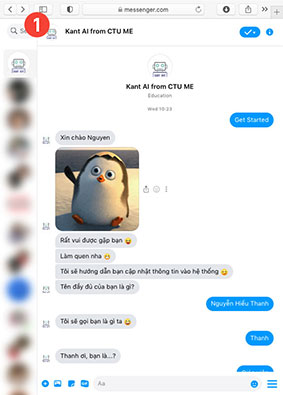
\includegraphics[width=7cm]{kant-ux/chat-1}
	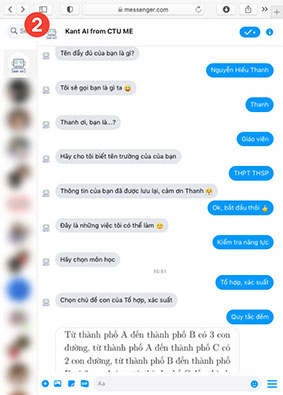
\includegraphics[width=7cm]{kant-ux/chat-2}
	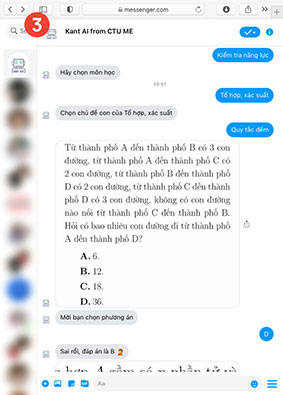
\includegraphics[width=7cm]{kant-ux/chat-3}
	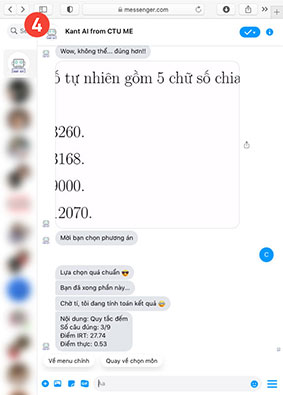
\includegraphics[width=7cm]{kant-ux/chat-4}
	\caption{Minh họa quá trình thực nghiệm với Kant}
	\label{fig:fig-c4-chatbot-demo}
\end{figure}\par

\subsubsection{Nội dung khảo sát}


